\subsection{НЕКОТОРЫЕ ЗАМЕЧАНИЯ}

В данном разделе будут даны некоторые замечания и описаны возможные объяснения тех мест описанного выше исследования, которые могли остаться не понятны.

\subsubsection{ВОСПРОИЗВОДИМОСТЬ РЕЗУЛЬТАТОВ}

В разделах \ref{sec:eff_mjo_gec}, \ref{sec:mjo_pg} и \ref{sec:futher_analysis} было показано, что КМД воздействует на интенсивность ГЭЦ постоянного тока. Было установлено, что моделируемый ИП и ГП, измеряемые в дни хорошей погоды на станции Восток, дают близкие к синусоидальным вариации по фазам КМД и имеют статистически значимую связь с индексами, характеризующими КМД.

Важно заметить, что вариации параметров ГЭЦ, представленные на рис. \ref{fig:variations}{a} и  \ref{fig:variations}{c}, не случайны. Аналогично рис. \ref{fig:variations}{a}, рис. \ref{fig:ip_pg_variation_partial}{a}--\ref{fig:ip_pg_variation_partial}{d} демонстрируют вариацию ИП по фазам КМД при усреднении не за весь 41 год моделирования, а при усреднении по различным десятилетиям. Хотя среднее значение ИП в каждое из десятилетий отличается от других, это не мешает наблюдать характерную близкую к синусоидальной вариацию ИП по фазам КМД в каждое из десятилетий.

\begin{figure}[htbp]
    \centering
    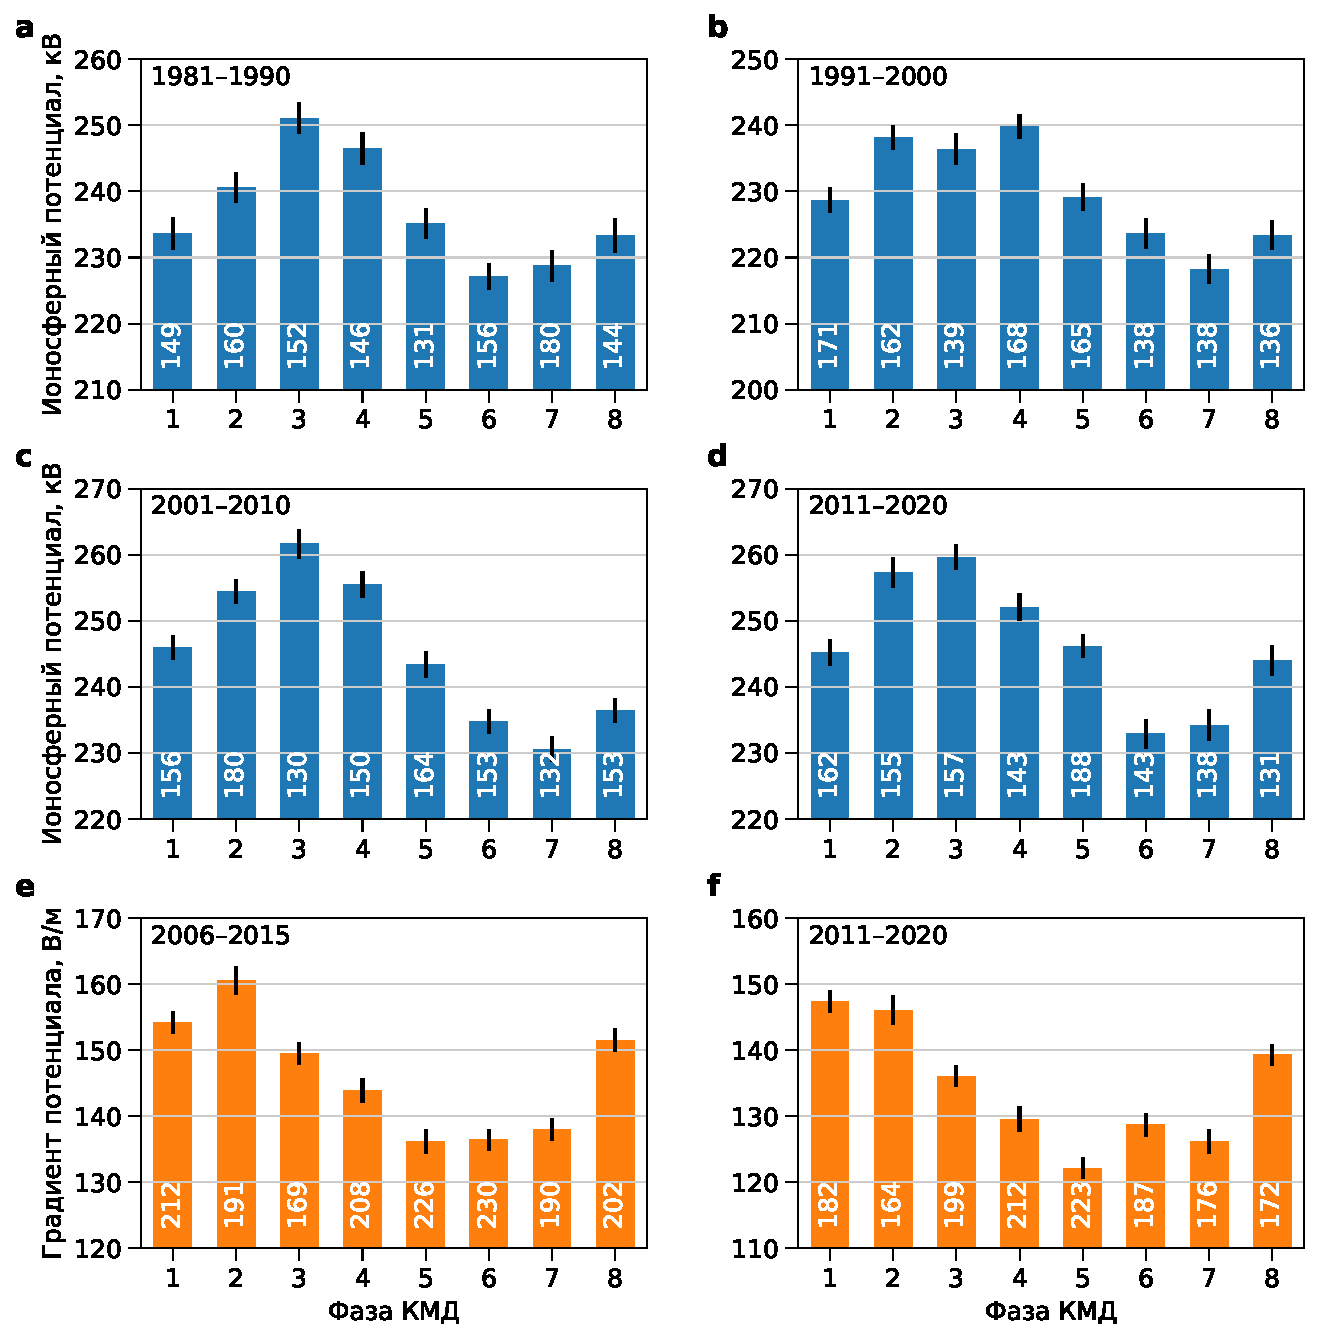
\includegraphics[width=\textwidth]{figures/ip_pg_variation_partial.pdf}
    \caption{(a)--(d): Усредненные значения ИП за каждую из фаз КМД на основе моделирования за 41 года (с 1 января 1980 года по 29 декабря 2020), первые четыре десятилетия рассмотрены раздельно. (e), (f): Средние значения ГП за дни хорошей погоды со станции Восток за каждую из фаз КМД на основе измерений в течение 2006--2015 и 2011--2020. Числа в столбцах означают, какое количество дней соответствует каждой из фаз КМД; черные штрихи на столбцах обозначают отклонение в одну стандартную ошибку.}
    \label{fig:ip_pg_variation_partial}
\end{figure}

Рис. \ref{fig:ip_pg_variation_partial}{e} и \ref{fig:ip_pg_variation_partial}{f} являются аналогами рис. \ref{fig:variations}{c} для двух перекрывающихся десятилетий 2006--2015 и 2011--2020. Из сравнения рис. \ref{fig:ip_pg_variation_partial}{e}, \ref{fig:ip_pg_variation_partial}{f} и \ref{fig:variations}{c}, видно, что форма вариации ГП по фазам КМД в целом не меняется (в случае 2011--2020 максимум сдвигается в первую фазу, однако значения ГП в первую и вторую фазу имеют перекрывающиеся интервалы стандартных ошибок), следовательно имеет универсальный характер.

Таким образом, получается выделить в ГЭЦ паттерны, явно связанные с КМД. Кроме исследований связей КМД с резонансами Шумана \cite{Anyamba_et_al_2000, Beggan_Musur_2019}, в литературе отсутствуют какие-либо исследования о воздействии КМД на электрическое окружение Земли. Учитывая недавно обнаруженную связь ЭНЮК с ГЭЦ постоянного тока \cite{Harrison_et_al_2011, Slyunyaev_et_al_2021a, Slyunyaev_et_al_2021b, Slyunyaev_et_al_2021c}, результаты данной работы позволяют подчеркнуть, что ГЭЦ является важной частью земной системы и отражает климатическую изменчивость, происходящую на различных временных масштабах. Стоит заметить, что параметры ГЭЦ как в случае с ЭНЮК, так и в случае с КМД требуют усреднения по многим событиям для обнаружения связей с рассматриваемыми климатическими модами.

\subsubsection{ЗАМЕЧАНИЯ ОТНОСИТЕЛЬНО ЭОФ-АНАЛИЗА}

Моделирование позволяет не только обнаружить эффект КМД в ГЭЦ, но и исследовать физический механизм, обеспечивающий наблюдаемый эффект. С данной целью ко вкладам экваториального региона, усредненным вдоль меридианов, был применен ЭОФ-анализ, который широко используется при исследовании КМД. ЭОФ задают базис пространственных паттернов, выбираемых таким образом, чтобы временные коэффициенты (ГК) разложения по первым нескольким из них, объясняли наибольшую возможную часть дисперсии. Это позволяет перейти от сложного исходного процесса к суперпозиции нескольких простых процессов.

Указанные в легенде рис. \ref{fig:eofs_and_pcs}{b} и \ref{fig:eofs_and_pcs}{e} числа обозначают объясняемую дисперсию каждой ЭОФ; если просуммировать эти числа, то окажется, что первые три ЭОФ объясняют лишь около 21\% исходной дисперсии. Не стоит удивляться столь малому проценту объясняемой дисперсии: дело в том, что вклады в ИП содержат изменчивость на многих масштабах, и большая часть этой изменчивости не имеет отношение к КМД. Данный факт можно продемонстрировать наглядным примером. На рис. \ref{fig:eofs_and_pcs}{d} изображен вклад в вариацию ИП от ЭОФ3$^\prime$. Видно, что вклад от данной ЭОФ в вариацию ИП по фазам КМД почти нулевой, хотя объясняемая дисперсия для ЭОФ3$^\prime$ составляет около 6\% --- значение, близкое к величинам объясняемой дисперсии ЭОФ1 (около 8\%) и ЭОФ2$^\prime$ (около 6\%), которые являются базовыми.

\subsubsection{ФАЗОВЫЙ СДВИГ МЕЖДУ ИП И ГП}
\label{sec:phase_shift}

Как показано в разделах \ref{sec:eff_mjo_gec} и \ref{sec:mjo_pg}, моделируемый ИП и измеряемый на станции Восток ГП за дни хорошей погоды имеют статистически значимую связь с циклом КМД. В то же время имеет место фазовый сдвиг между двумя такими параметрами ГЭЦ: ИП достигает максимального значения в третьей фазе КМД (см. рис. \ref{fig:variations}{a}) и имеет наибольший коэффициент корреляции с \eqref{rmm_direction} при $\phi = 290\text{\textdegree}$ (см. рис. \ref{fig:rmm_diagram}), а ГП достигает максимального значения во второй фазе (см. рис. \ref{fig:variations}{c}) и наиболее коррелирован с \eqref{rmm_direction} при $\phi = 225\text{\textdegree}$ (см. рис. \ref{fig:rmm_diagram}). 

Из теоретических соображений следует, что приповерхностный ГП в хорошую погоду связан с ИП соотношением \eqref{eq:pg_ip}. Такая формула напрямую отражает глобальный характер ГЭЦ: токи, обусловленные разделением зарядов в грозовых облаках и ESC по всей Земле, поднимаются вверх, обеспечивая вместе ИП, а затем стекают от ионосферы вниз к поверхности Земли через области хорошей погоды. Если пренебречь вариациями проводимости, то в хорошую погоду ГП прямо пропорционален ИП и отражает его динамику, как видно из \eqref{eq:pg_ip}. Однако в случае с КМД между измеряемым на станции Восток ГП и моделируемым ИП имеется фазовый сдвиг в примерно полторы фазы КМД, что не укладывается в рамки вышеописанного подхода. Ниже будут рассмотрены несколько наиболее вероятных причин, которые могли бы привести к наличию наблюдаемого сдвига.

Во-первых, к такому сдвигу могли привести ошибки параметризации ИП \eqref{eq:ip}. Возможно, вклады Морского континента и Восточной части Тихого океана в ИП переоцениваются рассматриваемой параметризацией \cite{Ilin_et_al_2020}. Учитывая тот факт, что ЭОФ1 описывает вклады в ИП в основном от Морского континента (см. рис. \ref{fig:eofs_and_pcs}{e}), такая переоценка могла бы привести к увеличению амплитуды изменчивости той части ИП, которая отвечает ЭОФ1. Если данная гипотеза верна, то при учете ошибки параметризации следует ожидать, что вариация ИП по фазам КМД в значительной степени будет складываться из вкладов, отвечающих ЭОФ2$^\prime$, что сдвинет максимум вариации ИП в сторону второй фазы.

Во-вторых, возможно, что наблюдаемое различие между ГП и ИП было вызвано различными факторами, влияющими на измерения ГП. Одним из таких факторов, влияющих на измерения ГП в Антарктике, является солнечная активность \cite{Burns_et_al_2017}. Солнечная активность влияет на процессы ионизации в атмосфере и тем самым возмущает проводимость воздуха (кроме того, солнечная активность может модулировать интенсивность источников ГЭЦ, но по данному вопросу ещё нет конечного понимания в мировом научном сообществе). Наиболее близкой к временным масштабам КМД (20--90 суток) является 27-дневный солнечный цикл, связанный со вращением Солнца вокруг своей оси. Естественно полагать, что 27-дневный солнечный цикл будет влиять на ГП на масштабах КМД. Следует отметить, что влияние солнечной активности на проводимость воздуха в рассматриваемой параметризации ИП \eqref{eq:ip} учтено не был, отсюда может проистекать наблюдаемое различие между вариациями ГП и ИП по фазам КМД.

% описать что вообще не так
% описать как текут токи, привести формулу, связывающую ГП в хорошую погоду и ИП пропорциональным соотнесением
% Рассмотреть вариант воздействия например ветра на измерения гп, для этого надо взять ветер на какой-нибудь низкой высоте, построить скаттер-плот мб, а самое главное посмотреть как коррелирует какой-нибудь параметр ветра с кмд или нет (типа главная гипотеза, которую ты здесь хочешь проверить --- дальняя связь КМД с ветром на станции восток дает фазовый сдвиг, хотя мб лучше вот как сделать: связан ли вообще этот ветер хоть как=то с кмд, если нет, то фуфло у тебя, а не гипотеза)